% ******************************* Plantilla mejorada para informes de laboratorio ECIM **************************
% Tecnológico de Costa Rica
\documentclass[letterpaper,12pt]{article}

%%%%%%%%%%%%
% Paquetes
%%%%%%%%%%%%
% Idioma y codificación
\usepackage[spanish]{babel}
\usepackage[utf8]{inputenc}
\usepackage[T1]{fontenc}

% Tipografía y espaciado
\usepackage{lmodern}
\usepackage{setspace}
\onehalfspacing

% Geometría de página
\usepackage{geometry}
\geometry{left=3cm,right=2cm,top=2.5cm,bottom=3cm}

% Encabezados y pies de página
\usepackage{fancyhdr}

% Autores
\usepackage{authblk}

% Matemática
\usepackage{amsmath,amssymb,amsfonts}

% Gráficos y figuras
\usepackage{graphicx}
\usepackage{caption}
\captionsetup[table]{position=bottom}
\addto\captionsspanish{\renewcommand{\tablename}{Tabla}}
\usepackage{caption,subcaption}

% Colores y tablas
\usepackage{xcolor,colortbl}
\usepackage{booktabs}
\usepackage{tabularx}
\usepackage{float}

% Unidades y química
\usepackage{siunitx}
\usepackage{mhchem}

% Hipervínculos
\usepackage{hyperref}
\hypersetup{
	colorlinks=true,
	linkcolor=black,
	urlcolor=blue,
	citecolor=black
}

% Otros
\usepackage{tcolorbox}
\usepackage{listings}
\usepackage{lipsum}

% Bibliografía
\usepackage[backend=biber,style=numeric,sorting=none]{biblatex}
\addbibresource{references.bib}

% Secciones un punto más grande
\usepackage{sectsty}
\sectionfont{\fontsize{14}{16}\selectfont}
\subsectionfont{\fontsize{13}{16}\selectfont}

%%%%%%%%%%%%%
% Estilo de ecuaciones
%%%%%%%%%%%%%
\numberwithin{equation}{section}

%%%%%%%%%%%%%
% Estilo encabezado
%%%%%%%%%%%%%
\pagestyle{fancy}
\lhead{
\includegraphics[width=30mm]{./images/ECIM.jpg}}
\rhead{
\includegraphics[width=30mm]{./images/ima3.jpg}}
\renewcommand{\headrulewidth}{0.4pt}

%%%%%%%%%%%%%
% Unidades personalizadas
%%%%%%%%%%%%%
\sisetup{output-decimal-marker = {,}, per-mode = symbol, list-units = brackets, range-phrase = --}
\DeclareSIUnit{\degreeFahrenheit}{\SIUnitSymbolDegree F}
\DeclareSIUnit{\uma}{uma}
\DeclareSIUnit{\ppm}{ppm}

%%%%%%%%%%%%%
% Titulo
%%%%%%%%%%%%%
\title{\bfseries Título del Laboratorio Realizado}
\author[1]{Primer Integrante}
\author[2]{Segundo Integrante}
\author[3]{Tercer Integrante}
\author[4]{Cuarto Integrante}
\author[5]{Quinto Integrante}
\renewcommand{\and}{ \unskip, }
\affil[1-5]{Escuela de Ciencia e Ingeniería en Materiales, Tecnológico de Costa Rica}

\date{\today}

%%%%%%%%%%%%%
\begin{document}
	\maketitle
	
	\begin{abstract}
		\noindent\rule{\textwidth}{0.4pt}
		\vspace{0.5em}
		
		El resumen es una versión condensada del informe, usualmente entre 100 y 200 palabras. Incluye el contexto, el problema abordado, la metodología empleada y los principales resultados/conclusiones.
		
		\vspace{0.5em}
		\noindent\rule{\textwidth}{0.4pt}
	\end{abstract}
	
	%%%%%%%%%%%%%%%
	\section{Introducción}
	Esta sección presenta el marco contextual, importancia del experimento y fundamentos científicos.  
	Por ejemplo, se pueden citar referencias así: \cite{Cooper2009}, \cite{Lozano2010}.  
	Para artículos científicos: \cite{young:1902}, \cite{Maity}.
	
	%%%%%%%%%%%%%%%
	\section{Objetivos}
	\subsection{Objetivo General}
	Expone el objetivo principal del experimento.
	
	\subsection{Objetivos Específicos}
	Lista concreta de acciones para alcanzar el objetivo general.
	
	%%%%%%%%%%%%%%%
	\section{Marco Teórico}
	Describe los conceptos relevantes al experimento, redactados con palabras propias y respaldados con citas.
	
	%%%%%%%%%%%%%%%
	\section{Materiales y Métodos}
	Describe procedimientos, condiciones experimentales y equipos utilizados. Incluye esquemas, fotos y cálculos representativos.
	
	\begin{tcolorbox}[colback=blue!5!white,colframe=blue!50!black,title=Ejemplo de cálculo]
		\begin{equation}
			E = E^0 - \frac{0.05916}{2} \log_{10} \left( \frac{[\ce{H+}]^2 F_{\ce{H2A}}}{[\ce{H+}]^2 + [\ce{H+}]K_1 + K_1 K_2} \middle/ F_D [\ce{H+}]^2 \right)
		\end{equation}
	\end{tcolorbox}
	
	%%%%%%%%%%%%%%%
	\section{Resultados y Análisis}
	Presenta resultados en tablas, gráficas, observaciones experimentales y comparación con literatura.
	
	\begin{table}[H]
		\centering
		\begin{tabularx}{0.95\textwidth}{X X X X}
			\toprule
			\textbf{Compuesto} & \textbf{Exp. (\si{\degreeCelsius})} & \textbf{Corregido (\si{\degreeCelsius})} & \textbf{Literatura (\si{\degreeCelsius})} \\
			\midrule
			Tolueno & 105 & 110 & 110,6 \\
			Ciclohexano & 76 & 81 & 80,7 \\
			\bottomrule
		\end{tabularx}
		\caption{Puntos de ebullición de muestras}
	\end{table}
	
	\begin{figure}[H]
		\centering
		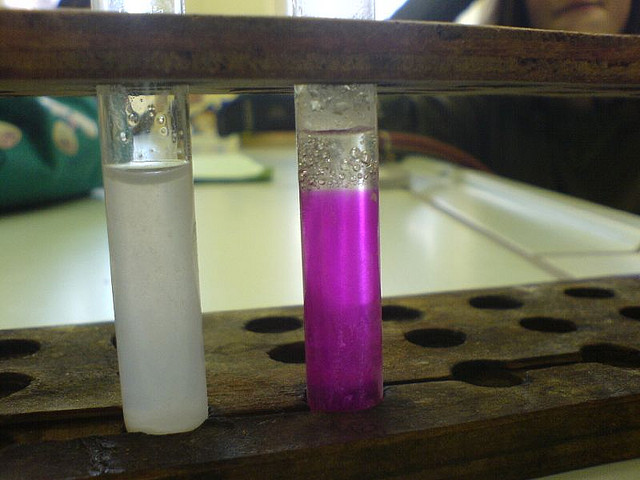
\includegraphics[width=0.6\linewidth]{images/tubes.jpg}
		\caption{Resultados del ensayo de insaturación}
		\label{fig:tubes}
	\end{figure}
	
	\subsection{Corrección por presión}
	\begin{equation}
		\Delta T = C(760 - p)(273 + t)
		\label{eq:bpcorrection}
	\end{equation}
	
	%%%%%%%%%%%%%%%
	\section{Conclusiones}
	\begin{itemize}
		\item Resume los hallazgos clave.
		\item Compara resultados con literatura.
		\item Sugiere mejoras o investigaciones futuras.
		\item Ejemplo de segundo orden:
		\begin{itemize}
			\item Esta viñeta es de segundo nivel y es un punto más pequeña.
			\item Todas las viñetas anidadas tienen el tamaño ajustado automáticamente.
		\end{itemize}
	\end{itemize}
	
	%%%%%%%%%%%%%%%
	\section{Referencias}
	\printbibliography
	
	%%%%%%%%%%%%%%%
	\newpage
	\section{Anexos}
	% Colocar gráficas, cálculos o datos adicionales aquí
	
	\begin{table}[H]
		\centering
		\begin{tabular}{|l|c|c|}
			\hline
			\textbf{Item a evaluar} & \textbf{Valor} & \textbf{Valor Obtenido} \\
			\hline
			Presentación & 5\% & \\
			\hline
			Resumen & 5\% & \\
			\hline
			Introducción & 10\% & \\
			\hline
			Objetivos & 10\% & \\
			\hline
			Marco Teórico & 10\% & \\
			\hline
			Materiales y Métodos & 10\% & \\
			\hline
			Resultados y Discusión & 30\% & \\
			\hline
			Conclusiones & 15\% & \\
			\hline
			Referencias Bibliográficas & 5\% & \\
			\hline
		\end{tabular}
		\caption{Rúbrica de evaluación}
	\end{table}
	
\end{document}
